It has as general purpose \tB{to find the right sample number}.
\begin{figure}[H]
    \begin{center}
        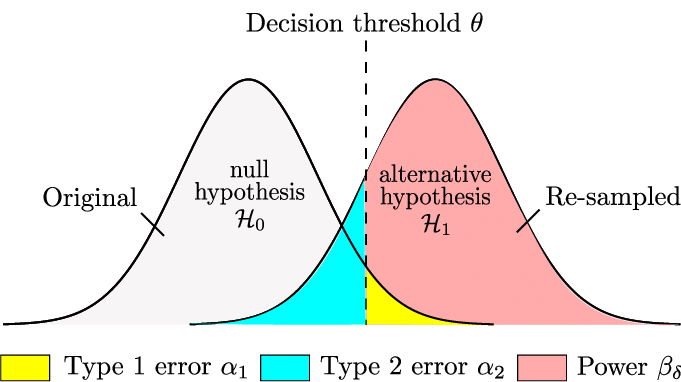
\includegraphics[width=\textwidth]{./chapters/2_statistics/04_frequentist_approach/6_images/1_statistical_hypothesis_testing.png}
    \end{center}
    \caption{caption}
    \label{fig:4.6.1_statistical_hypothesis_testing}
\end{figure}

\begin{center}
    \begin{tabular}{*{3}{|c}|}
    \hline
    & \textbf{$H_{0}$ \emph{is True}} & \textbf{$H_{1}$ \emph{is True}}\\
    \hline
        \textbf{Do not reject $H_{0}$} & \tG{Right decision} & \tR{Type II Error 
        \~{} $\beta$}\\
    \hline
        \textbf{Reject $H_{0}$} & \tR{Type I Error \~{} $\alpha$} & \tG{Right decision}\\
    \hline
    \end{tabular}
\end{center}

\paragraph{Power of the test}
Start by defining: \tB{$Power = 1-\beta$}, considering $H_{1}$ true it is the probability 
to correctly reject $H_{0}$

\paragraph{Significant threshold}
Then propose \tB{$\alpha$, the probability to wrongly reject $H_{0}$}. It will be the
reference to which the \emph{p-value} will be compared, \uB{the statistical test will be 
significant ($H_{0}$ rejected) if $\text{\emph{p-value}} \leq \alpha$}.

\paragraph{Effect size}
\uB{It quantifies how meaningful the relationship between variables or the difference 
between group is}, it indicates a practical significance.\\
\tB{While statistical significance (\emph{p-value}) shows the existence of an effect, 
practical significance (\emph{effect size}) shows if this effect is large enough to be 
meaningful in the real world.}\\
There are dozens of measures for effect sizes, and the most common are \emph{Cohen's d} 
and \emph{Pearson's r}.

\paragraph{Type of tests}
